\documentclass[english]{beamer}\usepackage[]{graphicx}\usepackage[]{color}
%% maxwidth is the original width if it is less than linewidth
%% otherwise use linewidth (to make sure the graphics do not exceed the margin)
\makeatletter
\def\maxwidth{ %
  \ifdim\Gin@nat@width>\linewidth
    \linewidth
  \else
    \Gin@nat@width
  \fi
}
\makeatother

\definecolor{fgcolor}{rgb}{0.345, 0.345, 0.345}
\newcommand{\hlnum}[1]{\textcolor[rgb]{0.686,0.059,0.569}{#1}}%
\newcommand{\hlstr}[1]{\textcolor[rgb]{0.192,0.494,0.8}{#1}}%
\newcommand{\hlcom}[1]{\textcolor[rgb]{0.678,0.584,0.686}{\textit{#1}}}%
\newcommand{\hlopt}[1]{\textcolor[rgb]{0,0,0}{#1}}%
\newcommand{\hlstd}[1]{\textcolor[rgb]{0.345,0.345,0.345}{#1}}%
\newcommand{\hlkwa}[1]{\textcolor[rgb]{0.161,0.373,0.58}{\textbf{#1}}}%
\newcommand{\hlkwb}[1]{\textcolor[rgb]{0.69,0.353,0.396}{#1}}%
\newcommand{\hlkwc}[1]{\textcolor[rgb]{0.333,0.667,0.333}{#1}}%
\newcommand{\hlkwd}[1]{\textcolor[rgb]{0.737,0.353,0.396}{\textbf{#1}}}%
\let\hlipl\hlkwb

\usepackage{framed}
\makeatletter
\newenvironment{kframe}{%
 \def\at@end@of@kframe{}%
 \ifinner\ifhmode%
  \def\at@end@of@kframe{\end{minipage}}%
  \begin{minipage}{\columnwidth}%
 \fi\fi%
 \def\FrameCommand##1{\hskip\@totalleftmargin \hskip-\fboxsep
 \colorbox{shadecolor}{##1}\hskip-\fboxsep
     % There is no \\@totalrightmargin, so:
     \hskip-\linewidth \hskip-\@totalleftmargin \hskip\columnwidth}%
 \MakeFramed {\advance\hsize-\width
   \@totalleftmargin\z@ \linewidth\hsize
   \@setminipage}}%
 {\par\unskip\endMakeFramed%
 \at@end@of@kframe}
\makeatother

\definecolor{shadecolor}{rgb}{.97, .97, .97}
\definecolor{messagecolor}{rgb}{0, 0, 0}
\definecolor{warningcolor}{rgb}{1, 0, 1}
\definecolor{errorcolor}{rgb}{1, 0, 0}
\newenvironment{knitrout}{}{} % an empty environment to be redefined in TeX

\usepackage{alltt}

%% The most common packages are already included in:
\usetheme{biostat}
%%%%%%%%%%%%%%%%%%%%%%%%%%%%%%%%%%%%%%%%%%%%%%%%%%%%%%%% 
\usepackage{amsmath,amsfonts,tikz}
\usetikzlibrary{trees}

%% Header data: (adjust to your needs:
\def\uzhunit{Biostatistics}             %% if (not) needed comment/uncomment
%\def\uzhunitext{STA480}

\title{Publication Bias in the Cochrane Library of Systematic Reviews}
%% Optional Argument in [Brackets]: Short Title for Footline

%% The following are all optional, simply comment them
%\subtitle{Subtitle (optional)}
%\institute{Biostatistics Journal Club}  %% optional
\author{Giuachin Kreiliger}
%\date{\today}
%%%%%%%%%%%%%%%%%%%%%%%%%%%%%%%%%%%%%%%%%%%%%%%%%%%%%%%% 

%%%%%%%%%%%%%%%%%%%%%%%%%%%%%%%%%%%%%%%%%%%%%%%%%%%%%%%%
\IfFileExists{upquote.sty}{\usepackage{upquote}}{}
\begin{document}
\maketitle
%%%%%%%%%%%%%%%%%%%%%%%%%%%%%%%%%%%%%%%%%%%%%%%%%%%%%%%% 
%% Start with slides here: put them between `\begin{frame}` and `\end{frame}`





\begin{frame}{Cochrane Library}
Database of high-quality, systematic reviews in clinical science.

Currently $\sim$ 8,000 reviews, prepared by independent groups. 

Reviews are peer-reviewed and prepared after guidelines.
\end{frame}


\begin{frame}{Cochrane Library Dataset}
5,016 systematic reviews with studies published until 2018.

52,995 studies.

463,820 study results.
\end{frame}


\begin{frame}{Dataset Structure}

\begin{figure}
\tikzstyle{every node}=[draw=black,thick,anchor=west,scale=.65]
\tikzstyle{selected}=[draw=red,fill=red!30]
\tikzstyle{optional}=[dashed,fill=gray!50]
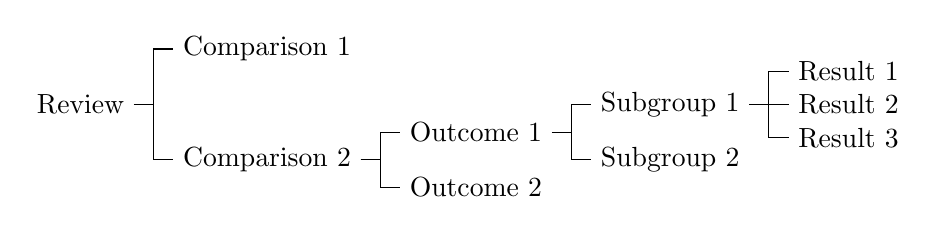
\begin{tikzpicture}
[grow = right, anchor = west,
  growth parent anchor=east, % added code
  parent anchor=east, level distance=.5cm,
  sibling distance=2em, level 1/.style={sibling distance=2em}, level 2/.style={sibling distance=2em},
  level 3/.style={sibling distance=2em}, level 4/.style={sibling distance=1.2em}]
  \node {Review} [edge from parent fork right]
    child { node {Comparison 2}
      child { node {Outcome 2}}
      child { node {Outcome 1}
        child { node {Subgroup 2}}
        child { node {Subgroup 1}
          child  { node {Result 3}}
          child  { node {Result 2}}
          child  { node {Result 1}}
          }}
    }
    child [missing] {}
    child { node {Comparison 1  }};
\end{tikzpicture}
%\caption{Structure of a hypothetical review with two different comparisons\label{review.structure}}
\label{review.structure}
\end{figure}

\end{frame}


\begin{frame}{Dataset Structure}
\begin{itemize}
\item Comparison: What is compared, e.g. treatment vs. control
\item Outcome: How it is compared
\item Subgroup: Subgroup affiliation
\item Meta-Analysis Group: Results from same comparison, outcome and subgroup
\end{itemize}
\end{frame}

\begin{frame}{Review Example: binary outcome}
Barbiturate efficacy in head injury
\vspace{-5mm}
% latex table generated in R 3.5.1 by xtable 1.8-3 package
% Sun May 12 21:11:51 2019
\begin{table}[ht]
\centering
\begingroup\tiny
\begin{tabular}{lllrrrr}
  \hline
Study & Comparison & Outcome & Events & Total & Events\_c & Total\_c \\ 
  \hline
Bohn 1989 & Barbiturate vs no b & Death at the end of & 11 & 41 & 11 & 41 \\ 
  Bohn 1989 & Barbiturate vs no b & Death or severe dis & 18 & 41 & 13 & 41 \\ 
  Eisenberg 1988 & Barbiturate vs no b & Uncontrolled ICP du & 25 & 37 & 30 & 36 \\ 
  Eisenberg 1988 & Barbiturate vs no b & Hypotension during  & 23 & 37 & 18 & 36 \\ 
  Perez-Barcena 2008 & Pentobarbital vs Th & Death at the end of & 16 & 21 & 9 & 21 \\ 
  Perez-Barcena 2008 & Pentobarbital vs Th & Death or severe dis & 17 & 21 & 13 & 21 \\ 
  Perez-Barcena 2008 & Pentobarbital vs Th & Uncontrolled ICP du & 18 & 22 & 11 & 22 \\ 
  Perez-Barcena 2008 & Pentobarbital vs Th & Hypotension during  & 20 & 22 & 21 & 22 \\ 
  Schwartz 1984 & Barbiturate vs Mann & Death at the end of & 6 & 15 & 7 & 14 \\ 
  Schwartz 1984 & Barbiturate vs Mann & Uncontrolled ICP du & 19 & 28 & 12 & 31 \\ 
  Ward 1985 & Barbiturate vs no b & Mean ICP during tre & 0 & 27 & 0 & 26 \\ 
  Ward 1985 & Barbiturate vs no b & Mean arterial press & 0 & 27 & 0 & 26 \\ 
  Ward 1985 & Barbiturate vs no b & Mean body temperatu & 0 & 27 & 0 & 26 \\ 
   \hline
\end{tabular}
\endgroup
\label{barbiturates}
\end{table}


% \vspace{-6mm}
% echo = FALSE, results = 'asis'>>=
% print(xtable(barbi1, label = "barbiturate.row", digits = 0),
%       include.rownames = F, size = "tiny")
% @

\end{frame}

\begin{frame}{Dataset Properties}
Missing data:
% latex table generated in R 3.5.1 by xtable 1.8-3 package
% Sun May 12 21:11:51 2019
\begin{table}[ht]
\centering
\begin{tabular}{lr}
  \hline
  \hline
Missing mean values and mean differences & 984 \\ 
  Missing standard deviations and standard errors & 1300 \\ 
  Missing sample sizes & 12173 \\ 
  Missing study year & 44649 \\ 
   \hline
\end{tabular}
\end{table}

\end{frame}


\begin{frame}{Dataset Properties}
Review and study properties:
% latex table generated in R 3.5.1 by xtable 1.8-3 package
% Sun May 12 21:11:51 2019
\begin{table}[ht]
\centering
\begingroup\footnotesize
\begin{tabular}{lrrrr}
  & 5\% quantile & median & mean & 95\% quantile \\ 
  \hline
Study number & 1 & 7 & 12 & 40 \\ 
   \hline
\hline
Comparison number & 1 & 2 & 4 & 12 \\ 
  Group number & 2 & 19 & 37 & 132 \\ 
  Study years & 1981 & 2002 & 2000 & 2013 \\ 
   \hline
Study sample size & 13 & 78 & 750 & 890 \\ 
  \end{tabular}
\endgroup
\end{table}

\end{frame}


\begin{frame}{Pooling Studies - Meta-Analysis}
Multiple results in a meta-analysis group can be pooled:

% latex table generated in R 3.5.1 by xtable 1.8-3 package
% Sun May 12 21:11:51 2019
\begin{table}[ht]
\centering
\begingroup\footnotesize
\begin{tabular}{rrr}
  \hline
n & Number of groups & Cumulative sum of groups \\ 
  \hline
1 & 102344 & 188079 \\ 
  2 & 31686 & 85735 \\ 
  3 & 16072 & 54049 \\ 
  4 & 9628 & 37977 \\ 
  5 & 6444 & 28349 \\ 
  6 & 4230 & 21905 \\ 
  7 & 2961 & 17675 \\ 
  8 & 2114 & 14714 \\ 
  9 & 1592 & 12600 \\ 
  10 & 11008 & 11008 \\ 
   \hline
\end{tabular}
\endgroup
\label{repr.groups}
\end{table}



\end{frame}

\begin{frame}{Meta-analysis}
Benefits:
\begin{itemize}
\item Summary of evidence (e.g. of a treatment)
\item More reliable evidence (?)
\end{itemize}

Assumptions:
\begin{itemize}
\item Identical study settings (can be relaxed)
\item Random sample of studies
\end{itemize}

\end{frame}

\begin{frame}{Small Study Effects}
``The tendency for the smaller studies to show larger treatment effects'' \citep{Sterne}
\end{frame}

\begin{frame}{Small Study Effects}
Causes:
\begin{itemize}
\item Selective publication of studies with large effects
\item Bias in smaller studies
\item Systematical differences in study settings
\item \ldots
\end{itemize}
\end{frame}

\begin{frame}{Publication Bias Tests}
Test for funnel plot asymmetry:

\vspace{-1cm}
\begin{figure}
\begin{knitrout}
\definecolor{shadecolor}{rgb}{0.969, 0.969, 0.969}\color{fgcolor}
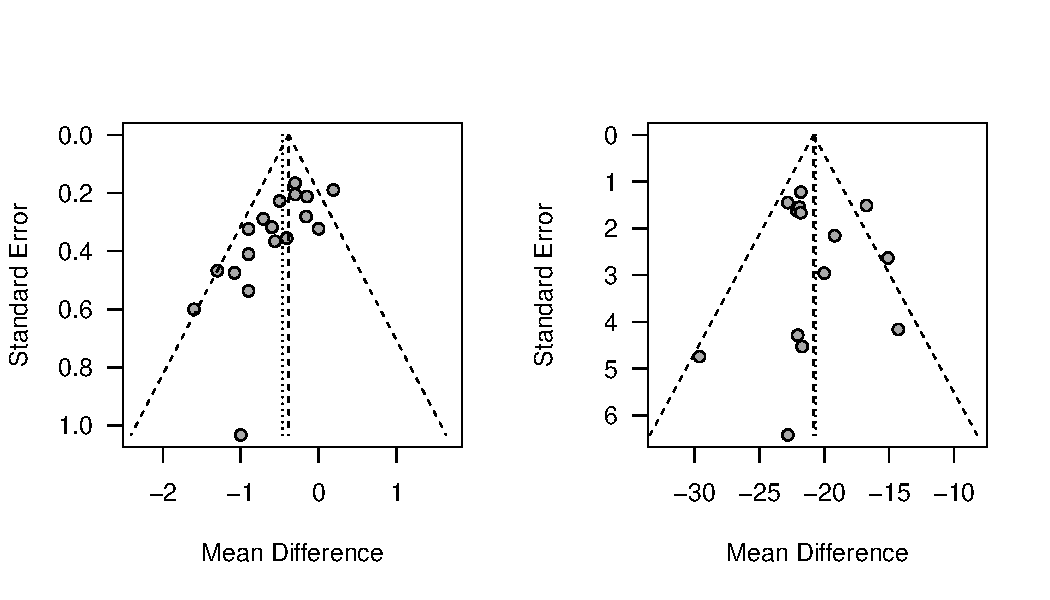
\includegraphics[width=\maxwidth]{figure/unnamed-chunk-6-1} 

\end{knitrout}
\end{figure}
\end{frame}

\begin{frame}{Publication Bias Tests}
Critical: Number of studies in meta-analysis must be large ($\geq$ 10).

Various tests for meta-analyses with continuous and binary outcomes:

Regression based: Egger's, Peter's or Thompson and Sharp's test

Rank based: Begg and Mazumdar's Test
\end{frame}
% 
% \begin{frame}{Publication Bias in the Cochrane Library}
% Publication bias tests applied for any meta analysis with n > 10
% 
% \vspace{-1.7cm}
% \begin{figure}[fragile]
% <<echo=FALSE, fig.height = 3.1, fig.width = 6.5 >>=
% grid.arrange(p.bin, p.cont, ncol = 2)
% @
% \end{figure}
% \end{frame}
% 
% \begin{frame}{Publication Bias}
% 
% \begin{figure}
% <<echo=FALSE, fig.height = 3.2, fig.width = 6.5 >>=
% grid.arrange(pbias.time, pbias.ss, ncol = 2)
% @
% \end{figure}
% \end{frame}
% 
% 
% 
% \begin{frame}{Publication Bias Adjustment}
% Three approaches:
% 
% Trim-and-fill: Non-parametric
% 
% Copas: Selection modelling, estimation by sensitivity analysis
% 
% Regression: Estimation of a treatment effect with infinite sample size
% \end{frame}









\begin{frame}{References}
  \small
  \bibliographystyle{apalike}
\bibliography{illustration}
\end{frame}

%\appendix
%% Possible backup slides...

%% chapter division is accomplished with:
%% \part{Appendix}

\end{document}
